%%
\chapter{Metoda zrealizowania pracy}
%%
Realizacja pracy będzie się opierać na opracowaniu kroków, które należy podjąć aby stworzyć świat gry w stylu low-poly. Dodatkowo aby zaprezentować stworzone elementy, zostanie opracowane przedstawienie produktu za pomocą projektu gry komputerowej stworzonej w Unity.
%%
%%
\section{Narzędzia badawcze}
\begin{itemize}
\item Pierwszym narzędziem badawczym do stworzenia obiektów, będzie program Blender, który idealnie nadaje się do tworzenia elementów grafiki 3D,

\item drugim narzędziem badawczym, które posłuży do stworzenia gry komputerowej będzie środowisko Unity, w którym zostaną zaprogramowane podstawowe elementy rozgrywki,

\item trzecim narzędziem badawczym, dzięki któremu napiszemy kod do gry, będzie Microsoft Visual Studio 2017.

\end{itemize}
%%

\section{Technika tworzenia obiektów 3D}
\indent Obiekty grafiki 3D o mianie low-poly określa się przedmioty, postacie, świat gry itp. na których widać wyraźne elementy trisów bądź poligonów. Są to wyraźnie zaznaczone krawędzie obiektu, które swoją geometrią przypominają odpowiednik w świecie rzeczywistym, jednakże różnią się stopniem skomplikowania obiektu. Aby stworzyć taki model, najłatwiej jest zacząć od projektów poglądowych. W studiach gier, zazwyczaj zatrudnieni sią artyści, którzy podczas omawiania aspektów danych postaci bądź elementów świata, rysują proste szkice, które następnie poprawiają w celu uwydatnienia kluczowych aspektów obiektu. 
W późniejszym stadium rozwoju danego elementu, powstaje tzw. szkic końcowy. Wówczas owy szkic przekazuje się osobom, które zajmują się grafiką komputerową aby stworzyli dany obiekt w środowisku 3D. Do tego projektu użyłem zdjęć poglądowych dla beczki, oraz słupka drogowego.

\indent Tworząc obiekt zazwyczaj zaczyna się od zwykłej kostki sześciennej, którą następnie modyfikuje się, poprzez przesuwanie vertexów, krawędzi bądź całych ścian obiektu. Istnieje wiele narzędzi w Blenderze, które pomagają uzyskać porządany przez nas efekt takie jak Mirror. Dodając ten modyfikator na obiekt, otrzymujemy odbicie lustrzane ukazujące dwie identyczne połówki. Korzystając ze zdjęcia referencyjnego ustawionego w widoku side view (bocznym) możemy ustawiać krawędzie obiektu nadając mu identyczny kształt jak na zdjęciu. Samochód który będzie głównym pojazdem w projekcie został stworzony za pomocą zdjęcia poglądowego Poloneza oraz własnej wyobraźni, ponieważ jego proporcje oraz kształt są niczym wyjęte z kreskówki. Obiekty stworzone w Blenderze, zostały wyeksportowane jako plik typu fbx.

\begin{figure}[!h]
\setcaptionwidth{0.5\linewidth}
\centering
  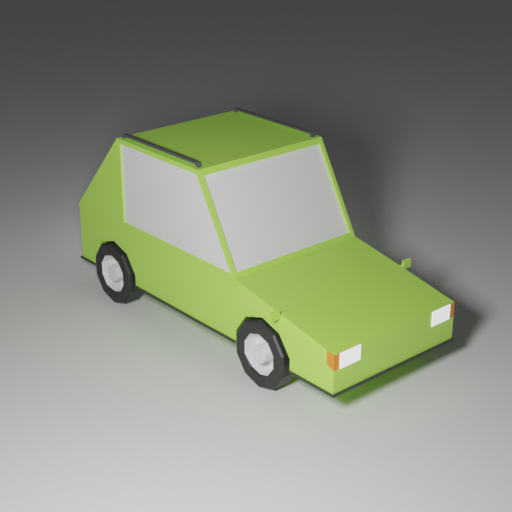
\includegraphics[width=0.5\linewidth]{carblend.png}
  \caption{Render samochodu stworzonego na potrzeby projektu}\label{rys_2}
  \begin{minipage}[t]{0.5\linewidth}
    \emph{Źródło: Grzegorz Dzikowicki}
  \end{minipage}
\end{figure}


\section{Środowisko Unity}
\indent Po wcześniejszym stworzeniu obiektów w Blenderze, przeszedłem do tworzenia środowiska w Unity. Aby obiekty nie wisiały w powietrzu, została stworzona płaska powierzchnia o rozmiarach 15x3x1000 jednostek Unity. Następnie umieściłem wszystkie obiekty w scenie. Każdy z obiektów posiada komponenty Mesh Collider, który odpowiada za wykrywanie kolizji z innymi obiektami, oraz Rigidbody będący głównym elementem fizyki obiektów.  Zostały zmodyfikowane ich masy oraz rozmiary aby stworzyć dla nich "prefab". Prefabem nazywany jest ten sam obiekt, jednakże po ponownym umieszczeniu go w scenie posiada te same właściwości. Ustawiając obiekty na powierzchni, stworzyłem 5 różnych poziomów, które różnią się trudnością, odpowiednio od pierwszego do piątego, bardziej skomplikowane ułożenie przeszkód oraz ich ilość. 

\indent Przejścia pomiędzy poziomami będą zawierały krótką i prostą animację wyświetlającą wiadomość "LEVEL COMPLETE". Tworzenie animacji polega na stworzeniu Panelu z tekstem a następnie na osi czasu zmiany wartości alfy, tak aby napis oraz tło pojawiły się. W sekcji programowania znajduje się kod, odpowiedzialny za proces przejścia z jednego poziomu na drugi. 

\section{Programowanie skryptów}
\indent Programowanie zacząłem od stworzenia skryptu obsługującego poruszanie się pojazdem. Aby obiekt się poruszał, wykorzystałem komponent Rigidbody umieszczony na samochodzie. Korzystając z gotowych funkcji zawartch w Rigidbody, mianowicie AddForce(), można sprawić aby obiekt poruszał się w danym kierunku z określoną mocą.

\begin{figure}[!h]
\setcaptionwidth{0.75\linewidth}
\centering
  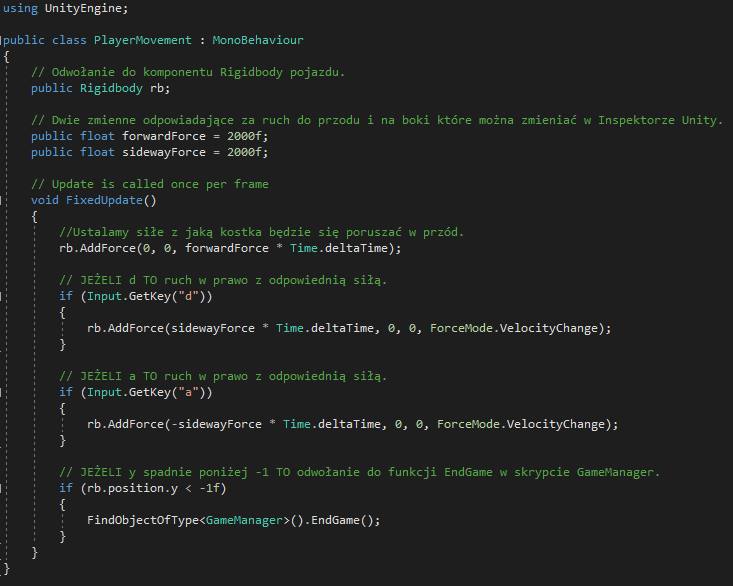
\includegraphics[width=1\linewidth]{playermove.png}
  \caption{Skrypt PlayerMovement obsługujący poruszanie się pojazdu po poziomie.}\label{rys_3}
  \begin{minipage}[t]{0.75\linewidth}
    \emph{Źródło: Grzegorz Dzikowicki}
  \end{minipage}
\end{figure}

\indent Kamera musi śledzić gracza, dlatego też napisałem skrypt, który ustala pozycję kamery w świecie gry, na taką samą pozycję co pojazd, jednakże dodawany jest offset, który podnosi kamerę do góry i przesuwa ją do tyłu, tak aby widok był z perspektywy trzeciej osoby.

\begin{figure}[!h]
\setcaptionwidth{0.75\linewidth}
\centering
  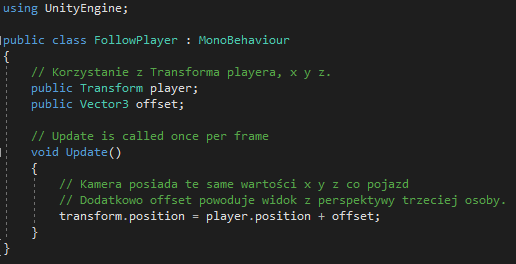
\includegraphics[width=1\linewidth]{followplayer.png}
  \caption{Skrypt FollowPlayer obsługujący umieszczenie kamery za pojazdem.}\label{rys_4}
  \begin{minipage}[t]{0.75\linewidth}
    \emph{Źródło: Grzegorz Dzikowicki}
  \end{minipage}
\end{figure}

\newpage
\indent Kolejnym przedsięwzięciem było napisanie skryptu, który będzie wykrywał kolizje z przeszkodami oraz resetował poziom, jeżeli pojazd spadnie z planszy. Ponieważ platforma po której porusza się pojazd, również jest wykrywana jako kolizja, wszystkie przeszkody zostały otagowane jako Obstacle. W skrypcie PlayerMovement został dodany kod obsługujący resetowanie poziomu, jeżeli wartość y pojazdu spadnie poniżej -1, który odwołuje się do funkcji EndGame w skrypcie GameManager.

\begin{figure}[!hbt]
\setcaptionwidth{0.75\linewidth}
\centering
  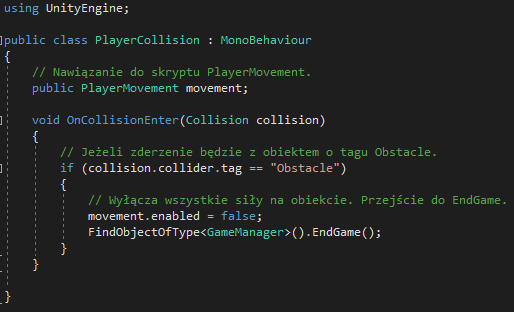
\includegraphics[width=1\linewidth]{playercollision.png}
  \caption{Skrypt PlayerCollision obsługujący kolizje pomiędzy pojazdem a przeszkodami.}\label{rys_5}
  \begin{minipage}[t]{0.75\linewidth}
    \emph{Źródło: Grzegorz Dzikowicki}
  \end{minipage}
\end{figure}
%%
\begin{figure}[!ht]
\setcaptionwidth{0.75\linewidth}
\centering
  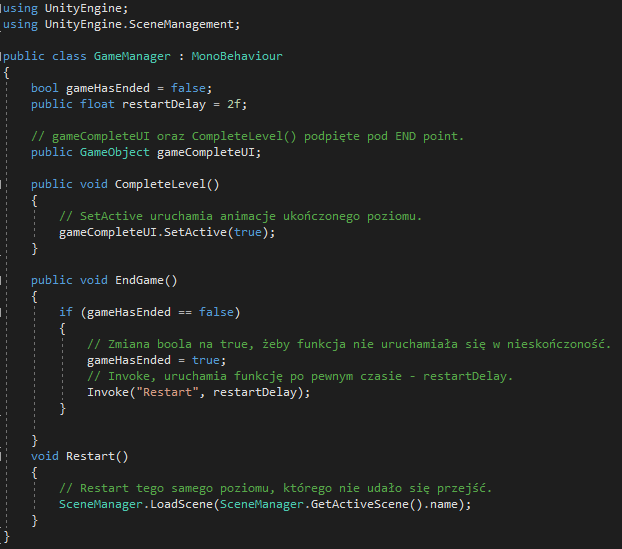
\includegraphics[width=1\linewidth]{gamemanager.png}
  \caption{Skrypt GameManager zajmujący się restowaniem poziomów.}\label{rys_6}
  \begin{minipage}[t]{0.75\linewidth}
    \emph{Źródło: Grzegorz Dzikowicki}
  \end{minipage}
\end{figure}

\indent Ponieważ w inspektorze nie da się podpiąć skryptu GameManager do prefabu pojazdu, w skrypcie PlayerCollision znajduje się metoda FindObjectOfType która przeszukuje w lokalizacji skryptów plik o nazwie GameManager a następnie korzysta z jego funkcji która musi być ustawiona jako public. Tworząc boola gameHasEnded, którego wartość zmieniana jest przy pierwszym uruchomieniu funkcji, upewniamy się, że funkcja będzie ładowana tylko jeden raz. Następnie po upadku, bądź kolizji, poziom jest ładowany od nowa, tak więc gameHasEnded ma swoją pierwotną wartość. Aby gra nie resetowała się za szybko, zamiast uruchamiać funkcję EndGame od razu, wykorzystałem metodę Invoke która po dodaniu nazwy funkcji, oraz czasu w sekundach, uruchamia funkcję po chwili. Aby przejść na następny poziom, musimy przejechać pomiędzy przeszkodami tak żeby ich nie dotknąć. W przypadku porażki poziom zostanie załadowany od nowa.

\indent Poziom jest już możliwy do przejścia, jednakże trzeba załadować kolejny. Na końcu trasy każdego z poziomów umieściłem kostkę o szerokości 15 jednostek Unity, która jest niewidoczna i służy jako Trigger, który uruchamia animację zakończonego poziomu, oraz ładuje kolejny. W skrypcie EndTrigger znajduje się jedna funkcja OnTriggerEnter(), która ładuje funkcję CompleteLevel() ze skryptu GameManager odpowiedzialną za włączenie animacji zakończenia poziomu.

\begin{figure}[!ht]
\setcaptionwidth{0.75\linewidth}
\centering
  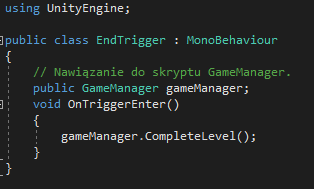
\includegraphics[width=1\linewidth]{endtrigger.png}
  \caption{Skrypt EndTrigger.}\label{rys_7}
  \begin{minipage}[t]{0.75\linewidth}
    \emph{Źródło: Grzegorz Dzikowicki}
  \end{minipage}
\end{figure}

\begin{figure}[!ht]
\setcaptionwidth{0.75\linewidth}
\centering
  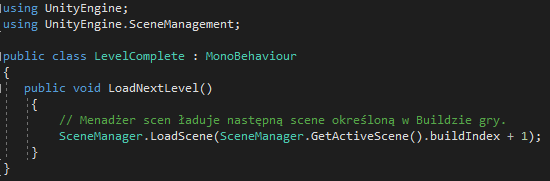
\includegraphics[width=1\linewidth]{loadlevel.png}
  \caption{Skrypt LevelComplete ładujący kolejny poziom.}\label{rys_8}
  \begin{minipage}[t]{0.75\linewidth}
    \emph{Źródło: Grzegorz Dzikowicki}
  \end{minipage}
\end{figure}

%%